% !TEX root = ../main.tex
\chapter{Estudio espectral del operador de multiplicación}\label{sec:estabilizacion}

En el Capítulo~\ref{sec:codimension_qk} construimos el marco abstracto de los índices $Q_k$. En este capítulo lo aplicamos al operador de multiplicación $\D p(z)=zp(z)$ y estudiamos la cadena de índices
\[
	Q_0(\D) \geq Q_1(\D) \geq Q_2(\D) \geq \dots
\]
cuando la norma proviene de un producto de Sobolev discreto de la forma
\begin{equation}\label{eq:norma_sobolev_discreta_general}
	\langle p,q\rangle_S
	=
	\int_{\mathbb{S}_R} p(z)\overline{q(z)}\,d\mathbf{m}_R(z)
	+
	\sum_{j=1}^N p'(c_j)\overline{q'(c_j)},
	\qquad p,q\in\Poly.
\end{equation}

La Figura~\ref{fig:geometria_atomos} resume la configuración geométrica asociada a \eqref{eq:norma_sobolev_discreta_general}.

\begin{figure}[H]
	\centering
	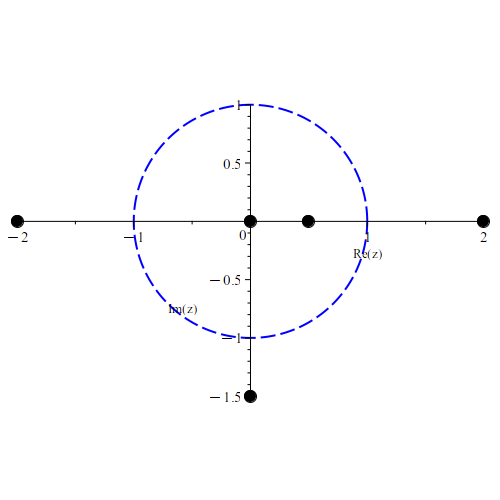
\includegraphics[width=0.35\linewidth]{figures/soporte_mixto}
	\caption{Configuración geométrica del soporte continuo $\mathbb{S}_R$ y de la posición de los átomos discretos.}
	\label{fig:geometria_atomos}
\end{figure}

Aunque a lo largo de esta memoria consideramos siempre, en la parte continua, la circunferencia unidad centrada en el origen, el siguiente resultado permite trasladar el estudio a cualquier otra circunferencia del plano complejo, pues la configuración geométrica del soporte se puede trasladar a nuestro caso mediante una transformación de semejanza.

\begin{prop}\label{prop:transformacion_afin_ch3}
	Sea $R>0$ y sea el producto de Sobolev discreto
	\[
		\langle p,q\rangle_S
		=
		\int_{\mathbb{S}_{a,R}} p(z)\overline{q(z)}\,d\mathbf{m}_{a;R}(z)
		+
		\sum_{j=1}^N p'(c_j)\overline{q'(c_j)},
		\qquad p,q\in\Poly.
	\]
	Sea $T(z)=\alpha z+\beta$ con $\alpha \in \mathbb{R}^+ \setminus \{0\}$ una semejanza, consideremos en $\Poly$ el operador \(U_Tp:=p\circ T^{-1}.\) Entonces el producto transportado por $U_T$ define un producto de Sobolev
	discreto $\langle \cdot,\cdot\rangle_T$ y $U_T$ es un isomorfismo isométrico.
\end{prop}

\begin{proof}
	Como $\alpha\neq 0$, la aplicación $T$ es biyectiva y
	\(
	T^{-1}(w)=\frac{w-\beta}{\alpha}.
	\)
	En particular, si $p\in\Poly$, entonces $U_Tp=p\circ T^{-1}$ es de nuevo un
	polinomio. Además, $U_T$ es lineal y biyectivo, con inversa
	\(
	U_T^{-1}P=P\circ T.
	\)

	Definimos el producto transportado por $U_T$ como
	\(
	\langle P,Q\rangle_T
	:=
	\langle U_T^{-1}P,U_T^{-1}Q\rangle_S
	\) para todo $P,Q\in\Poly$.

	De esta definición se deduce inmediatamente que
	$\langle\cdot,\cdot\rangle_T$ es sesquilineal y hermítico, pues
	$\langle\cdot,\cdot\rangle_S$ lo es y $U_T^{-1}$ es lineal. Además, si
	$P\neq 0$, entonces $U_T^{-1}P\neq 0$, y por tanto
	\(
	\langle P,P\rangle_T
	=
	\langle U_T^{-1}P,U_T^{-1}P\rangle_S
	>
	0.
	\)
	Así, $\langle\cdot,\cdot\rangle_T$ es un producto interno en $\Poly$.

	Veamos ahora que este producto tiene de nuevo la forma de un producto de
	Sobolev discreto. Sean $P,Q\in\Poly$. Como $U_T^{-1}P=P\circ T$ y
	$U_T^{-1}Q=Q\circ T$, tenemos
	\[
		\begin{aligned}
			\langle P,Q\rangle_T
			 & =
			\langle P\circ T,Q\circ T\rangle_S \\
			 & =
			\int_{\mathbb S_{a,R}}
			P(T(z))\overline{Q(T(z))}\,d\mathbf m_{a;R}(z)
			+
			\sum_{j=1}^N
			(P\circ T)'(c_j)\overline{(Q\circ T)'(c_j)}.
		\end{aligned}
	\]

	Calculamos primero la parte integral. Escribimos
	$\alpha=|\alpha|e^{i\theta}$. Entonces
	\[
		T(a+Re^{it})
		=
		T(a)+\alpha Re^{it}
		=
		T(a)+|\alpha|R e^{i(t+\theta)}.
	\]
	Por tanto, el cambio de variable $w=T(z)$ transforma la circunferencia
	$\mathbb S_{a,R}$ en la circunferencia
	$\mathbb S_{T(a),|\alpha|R}$. Además, al tratarse de medidas de arco
	normalizadas, el desfase angular $\theta$ no altera la medida. En efecto,
	para toda función continua $f$ en $\mathbb S_{T(a),|\alpha|R}$,
	\[
		\begin{aligned}
			\int_{\mathbb S_{a,R}} f(T(z))\,d\mathbf m_{a;R}(z)
			 & =
			\frac{1}{2\pi}
			\int_0^{2\pi}
			f(T(a+Re^{it}))\,dt                             \\
			 & =
			\frac{1}{2\pi}
			\int_0^{2\pi}
			f\bigl(T(a)+|\alpha|R e^{i(t+\theta)}\bigr)\,dt \\
			 & =
			\frac{1}{2\pi}
			\int_0^{2\pi}
			f\bigl(T(a)+|\alpha|R e^{it}\bigr)\,dt          \\
			 & =
			\int_{\mathbb S_{T(a),|\alpha|R}}
			f(w)\,d\mathbf m_{T(a);|\alpha|R}(w).
		\end{aligned}
	\]
	Aplicando esta identidad a $f(w)=P(w)\overline{Q(w)}$, obtenemos
	\[
		\int_{\mathbb S_{a,R}}
		P(T(z))\overline{Q(T(z))}\,d\mathbf m_{a;R}(z)
		=
		\int_{\mathbb S_{T(a),|\alpha|R}}
		P(w)\overline{Q(w)}\,d\mathbf m_{T(a);|\alpha|R}(w).
	\]

	Para la parte discreta, por la regla de la cadena,
	\[
		(P\circ T)'(z)=P'(T(z))T'(z)=\alpha P'(T(z)).
	\]
	En particular, para cada $j=1,\dots,N$,
	\[
		(P\circ T)'(c_j)=\alpha P'(T(c_j)),
		\qquad
		(Q\circ T)'(c_j)=\alpha Q'(T(c_j)).
	\]
	Por tanto,
	\[
		\begin{aligned}
			(P\circ T)'(c_j)
			\overline{(Q\circ T)'(c_j)}
			 & =
			\alpha P'(T(c_j))
			\overline{\alpha Q'(T(c_j))} \\
			 & =
			|\alpha|^2
			P'(T(c_j))\overline{Q'(T(c_j))}.
		\end{aligned}
	\]
	Sumando en $j=1,\dots,N$, se obtiene
	\[
		\sum_{j=1}^N
		(P\circ T)'(c_j)\overline{(Q\circ T)'(c_j)}
		=
		|\alpha|^2
		\sum_{j=1}^N
		P'(T(c_j))\overline{Q'(T(c_j))}.
	\]

	Sustituyendo las identidades anteriores en la expresión de
	$\langle P,Q\rangle_T$, queda
	\[
		\langle P,Q\rangle_T
		=
		\int_{\mathbb S_{T(a),|\alpha|R}}
		P(w)\overline{Q(w)}\,d\mathbf m_{T(a);|\alpha|R}(w)
		+
		|\alpha|^2
		\sum_{j=1}^N
		P'(T(c_j))\overline{Q'(T(c_j))}.
	\]
	Por tanto, el producto transportado es de nuevo un producto de Sobolev
	discreto, ahora sobre la circunferencia $\mathbb S_{T(a),|\alpha|R}$, con
	átomos $T(c_1),\dots,T(c_N)$ y peso $|\alpha|^2$.

	Finalmente, para cualesquiera $p,q\in\Poly$, por la propia definición del
	producto transportado,
	\[
		\langle U_Tp,U_Tq\rangle_T
		=
		\langle U_T^{-1}U_Tp,U_T^{-1}U_Tq\rangle_S
		=
		\langle p,q\rangle_S.
	\]
	Como $U_T$ es lineal y biyectivo, concluimos que $U_T$ es un isomorfismo
	isométrico entre
	$(\Poly,\langle\cdot,\cdot\rangle_S)$ y
	$(\Poly,\langle\cdot,\cdot\rangle_T)$.
\end{proof}

\begin{rmk}
	Si denotamos por
	\[
		\mathcal D_T P(w):=wP(w),
		\qquad P\in\Poly,
	\]
	el operador de multiplicación en el problema transformado, entonces
	\[
		U_T^{-1}\mathcal D_TU_T=\alpha\D+\beta I.
	\]
	En particular, si $(\varphi_n)_{n\ge 0}$ y $(\psi_n)_{n\ge 0}$ son las familias ortonormales asociadas a $\langle\cdot,\cdot\rangle_S$ y $\langle\cdot,\cdot\rangle_T$, respectivamente, entonces $\psi_n=\lambda_n\,U_T\varphi_n=\lambda_n\,\varphi_n\circ T^{-1}$ con $|\lambda_n|=1$, y por tanto los ceros se transportan por la misma semejanza.
\end{rmk}

\section{Propiedades de algunos funcionales de evaluación}

Los funcionales de evaluación y derivación aparecerán de forma recurrente en el análisis. En particular, el funcional asociado al operador de multiplicación jugará un papel central en la detección de las direcciones inestables.

\begin{defn}\label{def:funcionales_evaluacion_ch3}
	Para cada $c\in\C$ definimos inicialmente sobre $\Poly$ los funcionales lineales $\delta_c(p):=p(c)$ y $\delta'_c(p):=p'(c)$, con $p\in\Poly$, y el funcional asociado al operador de multiplicación
	\begin{equation}\label{eq:def_psi_c}
		\psi_c(p):=(\D p)'(c)=p(c)+cp'(c),
		\qquad p\in\Poly.
	\end{equation}
\end{defn}

\begin{rmk}
	Si alguno de estos funcionales es continuo respecto a la norma considerada, denotaremos por $\widetilde\delta_c$, $\widetilde\delta'_c$ o $\widetilde\psi_c$ su extensión continua a la compleción del espacio.
\end{rmk}

Veamos los siguientes resultados sobre la codimensión de intersecciones de núcleos de funcionales de evaluación.

\begin{lem}
	Sean $z_1,\dots,z_N\in\C$ distintos. Entonces $\delta_{z_1},\dots,\delta_{z_N}$ son linealmente independientes en $\Poly^*$.
\end{lem}

\begin{proof}
	Supongamos que existe una combinación lineal nula $\sum_{i=1}^N \alpha_i \delta_{z_i} = 0$.
	Para cada $j\in\{1,\dots,N\}$, sea
	\[
		L_j(z) = \prod_{\substack{l=1 \\ l \neq j}}^{N} \frac{z - z_l}{z_j - z_l}.
	\]
	Entonces $L_j(z_i)=\delta_{ji}$. Evaluando en $L_j$,
	\[
		0 = \sum_{i=1}^N \alpha_i \delta_{z_i}(L_j) = \sum_{i=1}^N \alpha_i L_j(z_i) = \alpha_j \cdot 1
	\]
	para todo $j$. Luego $\alpha_j=0$ para todo $j$.
\end{proof}

\begin{cor}
	Sean $z_1,\dots,z_N\in\C$ distintos y consideramos
	\(
	V:=\bigcap_{i=1}^N \ker(\delta_{z_i}).
	\)
	Entonces
	\[
		\operatorname{codim}_{\Poly}(V)=N.
	\]
\end{cor}

\begin{proof}
	Por el lema anterior, $\delta_{z_1},\dots,\delta_{z_N}$ son linealmente independientes. Aplicando la Proposición~\ref{prop:finite-codim-kernels},
	\(\operatorname{codim}_{\Poly}(V) = \dim[\delta_{z_1}, \dots, \delta_{z_N}] = N\).
\end{proof}

\begin{defn}\label{def:bpe_ch3}
	Sea $\mu$ una medida positiva finita en $\C$. Diremos que $a\in\C$ es un punto de evaluación acotada analítica (\emph{analytic bounded point evaluation}, $\operatorname{abpe}$) \cite{conway2020approximationmeanrationalfunctions,aleman2009nontangential} para $L^2(\mu)$ si existe un entorno abierto $U$ de $a$ y una constante $C>0$ tales que
	\[
		|p(z)|^2\le C\int |p(\zeta)|^2\,d\mu(\zeta),
		\qquad p\in\Poly,\ z\in U.
	\]
\end{defn}

\begin{defn}\label{def:delta_singular}
	Sea $\langle\cdot,\cdot\rangle_{\mu}$ un producto interno sobre $\Poly$. Diremos que un punto $c\in\C$ es \emph{$\delta$-singular} respecto a $\|\cdot\|_{\mu}$ si la restricción de $\delta_c$ a $\ker(\delta'_c)$ no es acotada, es decir,
	\[
		\sup\Bigl\{\frac{|p(c)|}{\|p\|_{\mu}}:p\in\ker(\delta'_c)\setminus\{0\}\Bigr\}=+\infty.
	\]
\end{defn}

\begin{rmk}
	La condición anterior es equivalente a la existencia de una sucesión $\{p_n\}_{n\ge1}$ con $p_n\in\ker(\delta'_c)$ tal que
	\[
		\|p_n\|_{\mu}\to0,
		\qquad
		p_n(c)=1
		\quad\text{para todo }n\ge1.
	\]
	En efecto, basta normalizar una sucesión para la que
	\[
		\frac{|p_n(c)|}{\|p_n\|_\mu}\to\infty.
	\]
\end{rmk}

\begin{lem}\label{lema:bpe_derivada}
	Sea $R>0$ y sea $c\in\C$ con $|c|<R$. Entonces $c$ es un punto $\operatorname{abpe}$ para $L^2(\mathbf{m}_R)$ y, en consecuencia, el funcional $\delta'_c(p)=p'(c)$, con $p\in\Poly$, es continuo respecto a la norma $L^2(\mathbf{m}_R)$.
\end{lem}

\begin{proof}
	En el caso de Lebesgue sobre la circunferencia, todo punto del disco abierto $\{|z|<R\}$ pertenece a $\operatorname{bpe}(\mathbf{m}_R)$ en el sentido de la Definición~\ref{def:bpe_intro}, y de hecho es $\operatorname{abpe}$ \cite{miller1999bounded,aleman2009nontangential}. Tomamos $r>0$ tal que la circunferencia $\gamma_r=\{z:|z-c|=r\}$ quede contenida en el disco $\{|z|<R\}$. Por la fórmula de Cauchy para la derivada,
	\[
		p'(c)=\frac{1}{2\pi i}\oint_{\gamma_r}\frac{p(z)}{(z-c)^2}\,dz.
	\]
	Luego $|p'(c)|\le \frac1r\max_{z\in\gamma_r}|p(z)|$. Como $\gamma_r\subset \operatorname{bpe}(\mathbf{m}_R)$ por la Definición~\ref{def:bpe_intro}, existe $M>0$ tal que $|p(z)|\le M\|p\|_{L^2(\mathbf{m}_R)}$ para $z\in\gamma_r$. Sustituyendo se obtiene $|p'(c)|\le \frac Mr\|p\|_{L^2(\mathbf{m}_R)}$.
	Esto prueba la continuidad de $\delta'_c$.
\end{proof}

Veamos algunas implicaciones de los puntos $\delta$-singulares para la acotación de los funcionales introducidos en la Definición \ref{def:funcionales_evaluacion_ch3} y luego su relación con la geometría del soporte de la medida de Lebesgue normalizada.

\begin{prop}\label{prop:caracterizacion_psi_c}
	Sea $\mu$ una medida positiva finita en $\C$, sea $c\in\C$ y sea $\psi_c(p)$ definido en \ref{eq:def_psi_c}, con $p\in\Poly$.
	Entonces se verifican las siguientes implicaciones:
	\begin{enumerate}
		\item Si $c$ es $\delta$-singular respecto a $\|\cdot\|_{\mu}$, entonces $\delta_c$ no es acotado sobre $\Poly$;
		\item Si $c$ es $\delta$-singular respecto a $\|\cdot\|_{\mu}$, entonces $\psi_c$ no es acotado sobre $\Poly$;
	\end{enumerate}
\end{prop}

\begin{proof}
	La primera implicación es inmediata, pues la no acotación de $\delta_c$ sobre $\ker(\delta'_c)$ implica su no acotación sobre el espacio mayor $\Poly$.

	Para la segunda, si $c$ es $\delta$-singular, existe una sucesión $\{p_n\}_{n\ge1}$ con $p_n \in \ker(\delta'_c)$ tal que $\|p_n\|_{\mu}\to0$ y $p_n(c)=1$.
	Como $p_n'(c)=0$, se tiene \(\psi_c(p_n)=p_n(c)=1\),
	y por tanto $\frac{|\psi_c(p_n)|}{\|p_n\|_{\mu}}=\frac1{\|p_n\|_{\mu}}\xrightarrow[n\to\infty]{}\infty$.
\end{proof}

\begin{thm}\label{thm:equivalencia_lebesgue}
	Sea $R>0$ y sea $c\in\C$. Consideremos la medida de Lebesgue normalizada $\mathbf{m}_R$ sobre $\mathbb{S}_R$. Entonces son equivalentes:
	\begin{enumerate}
		\item $c$ es $\delta$-singular respecto a $\|\cdot\|_{L^2(\mathbf{m}_R)}$;
		\item $|c|\ge R$.
	\end{enumerate}
\end{thm}

\begin{proof}
	Probamos primero que $(2)\Rightarrow(1)$. Si $|c|>R$, definimos
	\[
		r_n(z):=\frac{(n+1)c z^n-nz^{n+1}}{c^{n+1}}.
	\]
	Entonces $r_n(c)=1$, $r_n'(c)=0$ y
	\[
		\|r_n\|_{L^2(\mathbf{m}_R)}^2
		=
		(n+1)^2\left(\frac{R}{|c|}\right)^{2n}
		+
		n^2\left(\frac{R}{|c|}\right)^{2n+2}
		\xrightarrow[n\to\infty]{}0.
	\]
	Por tanto $c$ es $\delta$-singular.

	Si $|c|=R$, tomamos
	\[
		\alpha_n:=\frac{\sum_{k=1}^n k}{\sum_{k=1}^n k^2}=\frac{3}{2n+1},
		\qquad
		P_n(z):=\sum_{k=0}^n (1-\alpha_n k)\left(\frac zc\right)^k.
	\]
	Entonces $P_n'(c)=0$ y
	\[
		P_n(c)=\frac{(n+1)(n+2)}{2(2n+1)}.
	\]
	Definiendo $s_n:=P_n/P_n(c)$ se obtiene $s_n(c)=1$, $s_n'(c)=0$ y
	\[
		\|s_n\|_{L^2(\mathbf{m}_R)}^2
		=
		\frac{\|P_n\|_{L^2(\mathbf{m}_R)}^2}{|P_n(c)|^2}
		=
		\frac1{P_n(c)}
		\xrightarrow[n\to\infty]{}0.
	\]
	De nuevo $c$ es $\delta$-singular.

	Probamos ahora que $(1)\Rightarrow(2)$ por contrarrecíproco. Si $|c|<R$, entonces $c\in\operatorname{bpe}(\mathbf{m}_R)$ en el sentido de la Definición~\ref{def:bpe_intro} y, por el Lema~\ref{lema:bpe_derivada}, tanto $\delta_c$ como $\delta'_c$ son funcionales acotados respecto a $\|\cdot\|_{L^2(\mathbf{m}_R)}$. En particular, la restricción de $\delta_c$ a $\ker(\delta'_c)$ es acotada, y por ello $c$ no es $\delta$-singular.
\end{proof}

\begin{rmk}
	Nótese que para el producto de Sobolev discreto donde la parte continua es la medida de Lebesgue normalizada, los conjuntos de puntos $\operatorname{bpe}$ y $\delta$-singulares dividen el plano complejo en dos partes disjuntas, en el interior de la circunferencia y su complementario. Permitiendo tener una lectura geométrica de la pérdida de acotación del operador de multiplicación.
\end{rmk}

Gonzalo y Escribano \cite{EG25-2} tratan este caso en contextos más generales. A continuación presentamos un resultado particular correspondiente al producto de Sobolev discreto \eqref{eq:norma_sobolev_discreta_general}, usando que los puntos interiores son $\operatorname{abpe}$ para la parte continua.

\begin{prop}\label{prop:atomos_interiores_acotado}
	Sea $R>0$ y sean $c_1,\dots,c_N\in\C$ tales que $|c_j|<R$ para $j=1,\dots,N$.
	Consideremos sobre $\Poly$ el producto escalar
	\[
		\langle p,q\rangle_S
		=
		\int_{\mathbb{S}_R} p(z)\overline{q(z)}\,d\mathbf{m}_R(z)
		+
		\sum_{j=1}^N p'(c_j)\overline{q'(c_j)},
		\qquad p,q\in\Poly.
	\]
	Entonces $Q_0(\D)<\infty$.
\end{prop}

\begin{proof}
	Como $|c_j|<R$ para todo $j$, cada punto $c_j$ es $\operatorname{abpe}$ para $L^2(\mathbf{m}_R)$ y, por el Lema~\ref{lema:bpe_derivada}, la evaluación y la derivada en $c_j$ se controlan por la norma base. En consecuencia, para cada $j$ existen constantes $A_j,B_j<\infty$ tales que
	\[
		|p(c_j)|\le A_j\|p\|_{L^2(\mathbf{m}_R)},
		\qquad
		|p'(c_j)|\le B_j\|p\|_{L^2(\mathbf{m}_R)},
		\qquad p\in\Poly.
	\]
	Sea ahora $p\in\Poly$. Como $|z|=R$ sobre $\mathbb{S}_R$, $\|\D p\|_{L^2(\mathbf{m}_R)}=R\|p\|_{L^2(\mathbf{m}_R)}\le R\|p\|_S$.
	Además, para cada $j$,
	\[
		|(\D p)'(c_j)|=|p(c_j)+c_jp'(c_j)|
		\le
		(A_j+|c_j|B_j)\|p\|_{L^2(\mathbf{m}_R)}
		\le
		(A_j+|c_j|B_j)\|p\|_S.
	\]
	Por tanto,
	\[
		\|\D p\|_S^2
		=
		R^2\|p\|_{L^2(\mathbf{m}_R)}^2
		+
		\sum_{j=1}^N |(\D p)'(c_j)|^2
		\le
		\left(R^2+\sum_{j=1}^N (A_j+|c_j|B_j)^2\right)\|p\|_S^2.
	\]
	Esto prueba la acotación de $\D$, y por definición $Q_0(\D)=\|\D\|_S<\infty$.
\end{proof}

\begin{exm}\label{exm:c0_raiz2}
	La cota general del resultado anterior no es óptima en todos los casos. Tomemos $R=1$ y consideremos el producto escalar
	\[
		\langle p,q\rangle_S
		=
		\int_{\mathbb{S}_1} p(z)\overline{q(z)}\,d\mathbf m(z)
		+
		p'(0)\overline{q'(0)},
		\qquad p,q\in\Poly.
	\]
	Si $p(z)=\sum_{k=0}^n a_k z^k$, entonces $p'(0)=a_1$ y
	\begin{equation}\label{eq:norma_in_0}
		\|p\|_S^2=|a_0|^2+2|a_1|^2+\sum_{k=2}^n |a_k|^2.
	\end{equation}
	Además, para $\D p(z)=zp(z)$ se tiene $(\D p)'(0)=a_0$, luego
	\begin{equation}\label{eq:norma_out_0}
		\|\D p\|_S^2=2|a_0|^2+|a_1|^2+\sum_{k=2}^n |a_k|^2.
	\end{equation}
	Por tanto,
	\begin{equation}\label{eq:ratio_c0_raiz2}
		\frac{\|\D p\|_S^2}{\|p\|_S^2}
		=
		2-
		\frac{3|a_1|^2+\sum_{k\ge2}|a_k|^2}{\|p\|_S^2}
		\le2,
	\end{equation}
	y el máximo se alcanza en las funciones constantes. En consecuencia, $\|\D\|_S=Q_0(\D)=\sqrt2$.

	Por otra parte, si imponemos la restricción $p(0)=0$, entonces $a_0=0$ y las expresiones \eqref{eq:norma_in_0}--\eqref{eq:norma_out_0} dan $\|\D p\|_S^2=|a_1|^2+\sum_{k=2}^n |a_k|^2\le \|p\|_S^2$,
	de modo que sobre el subespacio $\ker(\delta_0)$ el operador actúa con norma a lo sumo $1$.
\end{exm}

Consideremos ahora el caso contrario, supongamos que existe al menos un punto $c_j$ con $|c_j|\ge R$. Para ilustrar este caso tomaremos un único átomo.

\begin{thm}\label{thm:un_atomo_exterior}\label{prop:lebesgue_pre_umbral_Qk}
	Sea $R>0$, sea $c\in\C$ con $|c|\ge R$ y consideremos sobre $\Poly$ el producto escalar
	\[
		\langle p,q\rangle_S
		=
		\int_{\mathbb{S}_R} p(z)\overline{q(z)}\,d\mathbf{m}_R(z)
		+
		p'(c)\overline{q'(c)},
		\qquad p,q\in\Poly.
	\]
	Entonces
	\[
		Q_0(\D)=\infty
		\qquad \text{y} \qquad
		Q_1(\D)\le R<\infty.
	\]
\end{thm}

\begin{proof}
	Por el Teorema~\ref{thm:equivalencia_lebesgue}, existe una sucesión $(p_n)\subset\Poly$ tal que
	\[
		p_n(c)=1,
		\qquad
		p_n'(c)=0,
		\qquad
		\|p_n\|_{L^2(\mathbf{m}_R)}\xrightarrow[n\to\infty]{}0.
	\]
	Como la parte discreta de la norma de Sobolev es $|p_n'(c)|^2=0$, se tiene también \(\|p_n\|_S\xrightarrow[n\to\infty]{}0\). Además, \(\psi_c(p_n)=p_n(c)+cp_n'(c)=1\).
	Por tanto, $\psi_c$ no es acotado respecto a $\|\cdot\|_S$.

	Además, \(|\psi_c(p)|=|(\D p)'(c)|\le \|\D p\|_S\) para todo \(p\in\Poly\).
	Si $\D$ fuese acotado, también lo sería $\psi_c$, contradicción. Luego $\D$ no es acotado y, por tanto,
	\(Q_0(\D)=\|\D\|_S=\infty\).

	Consideramos \(W:=\ker(\psi_c)=\{p\in\Poly:\psi_c(p)=0\}\).
	Este subespacio satisface $\operatorname{codim}_{\Poly}(W)=1$. Si $p\in W$, entonces
	\[
		\|\D p\|_S^2
		=
		\int_{\mathbb{S}_R}|zp(z)|^2\,d\mathbf{m}_R(z)
		+
		|\psi_c(p)|^2
	\]\[=
		\int_{\mathbb{S}_R}|zp(z)|^2\,d\mathbf{m}_R(z)
		\le
		R^2\int_{\mathbb{S}_R}|p(z)|^2\,d\mathbf{m}_R(z)
		\le
		R^2\|p\|_S^2.
	\]
	Por consiguiente, $\|\D|_W\|_S\le R$. Al tomar el ínfimo sobre los subespacios de codimensión algebraica menor que $2$, se obtiene
	\(
	Q_1(\D)\le R.
	\)
\end{proof}

Cuando consideremos $c_1,\dots,c_N\in\C$, reordenando los puntos si es necesario, fijamos un entero $m\in\{0,\dots,N\}$ tal que $|c_j|\ge R$ para $j=1,\dots,m$ y $|c_j|<R$ para $j=m+1,\dots,N$.

\begin{rmk}
	La Proposición~\ref{prop:atomos_interiores_acotado} resuelve el caso $m=0$. Por tanto, en los apartados posteriores supondremos cuando sea necesario que $m\ge1$.
	Por el Teorema~\ref{thm:equivalencia_lebesgue} y la Proposición~\ref{prop:caracterizacion_psi_c}, para cada $j=1,\dots,m$ el funcional $\psi_{c_j}$ no es acotado, mientras que los puntos $c_{m+1},\dots,c_N$ permanecen controlados por la parte continua.
\end{rmk}

\section{Acotación del operador de multipliacción en subespacios de codimensión finita}

En esta sección, construimos un subespacio de codimensión $m$ sobre el cual $\D$ es acotado, y después probamos que, con una codimensión estrictamente menor, el operador no puede estabilizarse.

Definimos ahora la notación del subespacio estable asociada al producto de Sobolev \eqref{eq:norma_sobolev_discreta_general}.
Sea $R>0$, sean $c_1,\dots,c_N\in\C$ y supongamos que $|c_j|\ge R$ para $j=1,\dots,m$ y $|c_j|<R$ para $j=m+1,\dots,N$.
Para cada $j=1,\dots,m$, denotamos por $\psi_{c_j}$ el funcional dado por \eqref{eq:def_psi_c} y escribimos
\begin{equation}\label{eq:def_vout}
	V_m:=\bigcap_{j=1}^m\ker(\psi_{c_j}).
\end{equation}

Veamos un resultado de interpolación de Hermite \cite{Dav75} que nos permitirá construir polinomios con valores y derivadas en un conjunto finito de puntos.

\begin{lem}\label{lem:hermite_datos_finito}
	Sea $F\subset\C$ un conjunto finito. Entonces, para cualesquiera familias de datos $(\alpha_a)_{a\in F}$ y $(\beta_a)_{a\in F}$ en $\C$, existe un polinomio $h\in\Poly$ tal que $h(a)=\alpha_a$ y $h'(a)=\beta_a$ para todo $a\in F$.
\end{lem}

\begin{lem}\label{lem:independencia_funcionales_psi}
	Sean $c_1,\dots,c_m\in\C$ distintos dos a dos. Entonces el sistema $\{\psi_{c_j}\}_{j=1}^m$ es linealmente independiente. En particular, $\dim[\psi_{c_1},\dots,\psi_{c_m}]=m$.
\end{lem}

\begin{proof}
	Fijado $j\in\{1,\dots,m\}$, aplicamos el Lema~\ref{lem:hermite_datos_finito} al conjunto $\{c_1,\dots,c_m\}$ con datos $\alpha_{c_k}=\delta_{jk}$ y $\beta_{c_k}=0$ para $k=1,\dots,m$. Obtenemos un polinomio $h_j\in\Poly$ tal que $h_j(c_k)=\delta_{jk}$ y $h_j'(c_k)=0$ para $k=1,\dots,m$. Entonces $\psi_{c_k}(h_j)=h_j(c_k)+c_kh_j'(c_k)=\delta_{jk}$ para $k=1,\dots,m$,
	y esto prueba la independencia lineal.
\end{proof}

\begin{lem}\label{lem:vout_codimension}
	Sea $R>0$, sean $c_1,\dots,c_N\in\C$ distintos dos a dos y sea $V_m$ definido en~\ref{eq:def_vout}. Entonces $$\operatorname{codim}_{\Poly}(V_m)=m$$.
\end{lem}

\begin{proof}
	Por definición, $V_m$ es una intersección finita de núcleos de funcionales lineales. El Lema~\ref{lem:independencia_funcionales_psi} muestra que los funcionales $\{\psi_{c_j}\}_{j=1}^m$ son linealmente independientes y generan un espacio de dimensión $m$. La Proposición~\ref{prop:finite-codim-kernels} da entonces la igualdad anunciada.
\end{proof}

\begin{lem}\label{lem:vout_acotacion}
	Sea $R>0$, sean $c_1,\dots,c_N\in\C$ distintos dos a dos y supongamos que $|c_j|\ge R$ para $j=1,\dots,m$ y $|c_j|<R$ para $j=m+1,\dots,N$. Consideramos $V_m$ introducido en ~\ref{eq:def_vout}, y el producto escalar
	\[
		\langle p,q\rangle_S
		=
		\int_{\mathbb{S}_R} p(z)\overline{q(z)}\,d\mathbf{m}_R(z)
		+
		\sum_{j=1}^N p'(c_j)\overline{q'(c_j)},
		\qquad p,q\in\Poly.
	\]
	Entonces $\|\D|_{V_m}\|_S$ es finita y $\|\D|_{V_N}\|_S\leq R$.
\end{lem}

\begin{proof}
	Sea $p\in V_m$. Entonces, para todo $j=1,\dots,m$, se tiene $(\D p)'(c_j)=\psi_{c_j}(p)=0$.

	Para cada $j=m+1,\dots,N$, como $|c_j|<R$, por el Lema~\ref{lema:bpe_derivada} y la propiedad $\operatorname{abpe}$ de los puntos interiores existen constantes $A_j,B_j<\infty$ tales que
	\[
		|p(c_j)|\le A_j\|p\|_S,
		\qquad
		|p'(c_j)|\le B_j\|p\|_S.
	\]
	De aquí se deduce
	\[
		|(\D p)'(c_j)|=|p(c_j)+c_jp'(c_j)|\le (A_j+|c_j|B_j)\|p\|_S.
	\]

	Además, como $|z|=R$ en $\mathbb{S}_R$, $\|zp\|_{L^2(\mathbf{m}_R)}\le R\|p\|_{L^2(\mathbf{m}_R)}\le R\|p\|_S$.
	Por consiguiente,
	\[
		\|\D p\|_S^2
		=
		\|zp\|_{L^2(\mathbf{m}_R)}^2
		+
		\sum_{j=m+1}^N |(\D p)'(c_j)|^2
		\le
		\left(R^2+\sum_{j=m+1}^N (A_j+|c_j|B_j)^2\right)\|p\|_S^2.
	\]
	Luego $\|\D|_{V_m}\|_S$ es finita. Si $m=N$, la suma anterior desaparece y queda $\|\D p\|_S^2\le R^2\|p\|_S^2$,
	de modo que se tiene $\|\D|_{V_N}\|_S\leq R$.
\end{proof}

\begin{prop}\label{prop:umbral_fase1}
	Sean $R>0$, $c_1,\dots,c_N\in\C$ distintos dos a dos y supongamos que $|c_j|\ge R$ para $j=1,\dots,m$ y $|c_j|<R$ para $j=m+1,\dots,N$. Consideramos $V_m$ introducido en~\ref{eq:def_vout} y el producto escalar
	\[
		\langle p,q\rangle_S
		=
		\int_{\mathbb{S}_R} p(z)\overline{q(z)}\,d\mathbf{m}_R(z)
		+
		\sum_{j=1}^N p'(c_j)\overline{q'(c_j)},
		\qquad p,q\in\Poly.
	\]
	Entonces $Q_m(\D)<\infty$ y $Q_N(\D) \leq R$
\end{prop}

\begin{proof}
	Por el Lema~\ref{lem:vout_acotacion}, la restricción $\D|_{V_m}$ es acotada. Tomando ínfimo sobre los subespacio se tiene inmediatamente
	\(Q_m(\D)\le \|\D|_{V_m}\|_S<\infty\). De manera análoga tenemos para \(Q_N(\D)\le \|\D|_{V_N}\|_S\le R\)
\end{proof}

Probamos ahora que la codimensión $m$ es necesaria para estabilizar el operador de multiplicación. Comenzamos con la construcción de las sucesiones auxiliares que serán utiles para la prueba del resultado.

\begin{lem}\label{lem:paquete_local_exterior}
	Sea $R>0$ y sea $c\in\C$ con $|c|\ge R$. Entonces existe una sucesión $(r_{c,n})_{n\ge1} \subset \Poly$ tal que
	\[
		r_{c,n}(c)=1,
		\qquad
		r'_{c,n}(c)=0,
		\qquad
		\|r_{c,n}\|_{L^2(\mathbf{m}_R)}\xrightarrow[n\to\infty]{}0.
	\]
\end{lem}

\begin{proof}
	Por el Teorema~\ref{thm:equivalencia_lebesgue}, la condición $|c|\ge R$ equivale a que $c$ es $\delta$-singular respecto a $\|\cdot\|_{L^2(\mathbf{m}_R)}$. La observación siguiente a la Definición~\ref{def:delta_singular} proporciona entonces una sucesión $(r_{c,n})_{n\ge1}\subset\Poly$ tal que
	\(r_{c,n}(c)=1\), \(r'_{c,n}(c)=0\) y \(\|r_{c,n}\|_{L^2(\mathbf{m}_R)}\xrightarrow[n\to\infty]{}0\).
\end{proof}

\begin{lem}\label{lem:paquetes_diagonales}
	Sea $R>0$, sean $c_1,\dots,c_N\in\C$ distintos dos a dos y supongamos que $|c_j|\ge R$ para $j=1,\dots,m$ y $|c_j|<R$ para $j=m+1,\dots,N$. Consideremos los funcionales $\psi_{c_k}$ definidos en \eqref{eq:def_psi_c}. Entonces, para cada $j=1,\dots,m$, existe una sucesión $(u_{j,n})_{n\ge1}\subset\Poly$ tal que
	\[
		\|u_{j,n}\|_S\xrightarrow[n\to\infty]{}0
		\qquad\text{y}\qquad
		\psi_{c_k}(u_{j,n})=\delta_{kj}
		\quad \forall k\in\{1,\dots,m\}.
	\]
\end{lem}

\begin{proof}
	Fijamos $j\in\{1,\dots,m\}$. Aplicamos el Lema~\ref{lem:hermite_datos_finito} al conjunto finito $\{c_1,\dots,c_N\}$ y obtenemos un polinomio $H_j\in\Poly$ tal que
	\[
		H_j(c_j)=1,
		\qquad
		H'_j(c_j)=0,
	\]
	y, para todo $k\in\{1,\dots,N\}\setminus\{j\}$,
	\[
		H_j(c_k)=0,
		\qquad
		H'_j(c_k)=0.
	\]
	Sea $(r_{c_j,n})_{n\ge1}$ la sucesión dada por el Lema~\ref{lem:paquete_local_exterior} y definamos
	\(
	u_{j,n}:=H_j\,r_{c_j,n}.
	\) Si $k=j$, entonces
	\[
		u_{j,n}(c_j)=H_j(c_j)r_{c_j,n}(c_j)=1
	\]
	y
	\[
		u'_{j,n}(c_j)=H'_j(c_j)r_{c_j,n}(c_j)+H_j(c_j)r'_{c_j,n}(c_j)=0.
	\]
	Por tanto,
	\(
	\psi_{c_j}(u_{j,n})=u_{j,n}(c_j)+c_j u'_{j,n}(c_j)=1.
	\) Si $k\in\{1,\dots,m\}\setminus\{j\}$, entonces $H_j(c_k)=H'_j(c_k)=0$, luego
	\(
	u_{j,n}(c_k)=0,
	\) y \(
	u'_{j,n}(c_k)=0,
	\) y por tanto \(
	\psi_{c_k}(u_{j,n})=0.
	\) En consecuencia,
	\[
		\psi_{c_k}(u_{j,n})=\delta_{kj},
		\qquad k=1,\dots,m.
	\]

	Además, para todo $k=1,\dots,N$, la elección de $H_j$ y $r_{c_j,n}$ da
	\[
		u'_{j,n}(c_k)
		=
		H'_j(c_k)r_{c_j,n}(c_k)+H_j(c_k)r'_{c_j,n}(c_k)
		=
		0.
	\]
	En consecuencia, todas las contribuciones discretas de la norma de Sobolev de $u_{j,n}$ se anulan y
	\(
	\|u_{j,n}\|_S^2=\|u_{j,n}\|_{L^2(\mathbf{m}_R)}^2.
	\)
	Como $H_j$ es fijo,
	\[
		\|u_{j,n}\|_{L^2(\mathbf{m}_R)}
		=
		\|H_j r_{c_j,n}\|_{L^2(\mathbf{m}_R)}
		\le
		\|H_j\|_{L^\infty(\mathbb{S}_R)}\,\|r_{c_j,n}\|_{L^2(\mathbf{m}_R)}.
	\]
	Por el Lema~\ref{lem:paquete_local_exterior}, el último término tiende a cero. Luego
	\(
	\|u_{j,n}\|_S\xrightarrow[n\to\infty]{}0.
	\)
\end{proof}

\begin{lem}\label{lem:imposicion_restricciones}
	Sea $R>0$, sean $c_1,\dots,c_N\in\C$ distintos dos a dos y supongamos que $|c_j|\ge R$ para $j=1,\dots,m$ y $|c_j|<R$ para $j=m+1,\dots,N$ con $m\ge1$.
	Consideremos $V\subset\Poly$ un subespacio con $\operatorname{codim}_{\Poly}(V)<m$ y $W_n:=[u_{1,n},\dots,u_{m,n}]$, donde $u_{j,n}$ son los polinomios obtenidos en el Lema~\ref{lem:paquetes_diagonales}. Entonces, para cada $n\ge1$, existe un polinomio no nulo $p_n\in V\cap W_n$ de la forma $p_n=\sum_{j=1}^m \alpha_j^{(n)}u_{j,n}$, con coeficientes normalizados por $\sum_{j=1}^m |\alpha_j^{(n)}|^2=1$.
\end{lem}

\begin{proof}
	Escribimos $\operatorname{codim}_{\Poly}(V)=r<m$. Existen entonces funcionales lineales independientes $L_1,\dots,L_r:\Poly\to\C$ tales que $V=\bigcap_{i=1}^r\ker(L_i)$.
	Para cada $n$ consideramos la matriz
	\[
		A_n:=\bigl(L_i(u_{j,n})\bigr)_{\substack{1\le i\le r\\ 1\le j\le m}}\in\C^{r\times m}.
	\]
	Como $r<m$, el núcleo de $A_n$ es no trivial. Elegimos $\alpha^{(n)}=(\alpha_j^{(n)})_{j=1}^m\in\ker(A_n)$ con $\|\alpha^{(n)}\|_{\ell^2}=1$, y definimos $p_n:=\sum_{j=1}^m \alpha_j^{(n)}u_{j,n}$.
	Entonces, para cada $i=1,\dots,r$,
	\[
		L_i(p_n)=\sum_{j=1}^m \alpha_j^{(n)}L_i(u_{j,n})=0,
	\]
	y por tanto $p_n\in V$. Además $p_n\in W_n$ por construcción.

	Resta ver que $p_n\neq0$. Si fuese $p_n=0$, entonces aplicando $\psi_{c_k}$ para un $k\in\{1,\dots,m\}$ obtendríamos $0=\psi_{c_k}(p_n)=\sum_{j=1}^m \alpha_j^{(n)}\psi_{c_k}(u_{j,n})=\alpha_k^{(n)}$.
	Como esto vale para todo $k=1,\dots,m$, se seguiría $\alpha^{(n)}=0$, contradiciendo la normalización $\|\alpha^{(n)}\|_{\ell^2}=1$.
\end{proof}

Ahora procedemos a probar uno de los resultados principales de este capítulo.

\begin{thm}\label{thm:umbral_fase2}\label{prop:umbral_fase2}
	Sea $R>0$, sean $c_1,\dots,c_N\in\C$ distintos dos a dos y supongamos que $|c_j|\ge R$ para $j=1,\dots,m$ y $|c_j|<R$ para $j=m+1,\dots,N$ con $m\ge1$. Consideremos sobre $\Poly$ el producto escalar
	\[
		\langle p,q\rangle_S
		=
		\int_{\mathbb{S}_R} p(z)\overline{q(z)}\,d\mathbf{m}_R(z)
		+
		\sum_{j=1}^N p'(c_j)\overline{q'(c_j)},
		\qquad p,q\in\Poly.
	\]
	Entonces
	\(
	Q_{m-1}(\D)=\infty.
	\)
\end{thm}

\begin{proof}
	Sea $V\subset\Poly$ con $\operatorname{codim}_{\Poly}(V)<m$. Para cada $n\ge1$ consideramos el subespacio $W_n:=[u_{1,n},\dots,u_{m,n}]$, donde los $u_{j,n}$ son los polinomios del Lema~\ref{lem:paquetes_diagonales}. Por el Lema~\ref{lem:imposicion_restricciones}, para cada $n$ existe un polinomio no nulo $p_n=\sum_{j=1}^m \alpha_j^{(n)}u_{j,n}\in V\cap W_n$ con $\sum_{j=1}^m |\alpha_j^{(n)}|^2=1$.

	Por el Lema~\ref{lem:paquetes_diagonales}, para cada $k=1,\dots,m$ se tiene
	\[
		\psi_{c_k}(p_n)=\sum_{j=1}^m \alpha_j^{(n)}\psi_{c_k}(u_{j,n})=\alpha_k^{(n)}.
	\]
	En consecuencia,
	\[
		\sum_{k=1}^m |\psi_{c_k}(p_n)|^2
		=
		\sum_{k=1}^m |\alpha_k^{(n)}|^2
		=
		1.
	\]
	Como $\psi_{c_k}(p_n)=(\D p_n)'(c_k)$, la parte discreta de la norma de Sobolev de $\D p_n$ satisface
	\[
		\|\D p_n\|_S^2\ge \sum_{k=1}^m |(\D p_n)'(c_k)|^2=1.
	\]
	Por otra parte,
	\[
		\|p_n\|_S
		\le
		\sum_{j=1}^m |\alpha_j^{(n)}|\,\|u_{j,n}\|_S
		\le
		\sqrt m\max_{1\le j\le m}\|u_{j,n}\|_S
		\xrightarrow[n\to\infty]{}0
	\]
	por el Lema~\ref{lem:paquetes_diagonales}. Por tanto,
	\[
		\frac{\|\D p_n\|_S}{\|p_n\|_S}\xrightarrow[n\to\infty]{}\infty,
	\]
	y la restricción $\D|_V$ no puede ser acotada. Como $V$ era arbitrario entre los subespacios de codimensión menor que $m$, concluimos que $Q_{m-1}(\D)=\infty$.
\end{proof}

\section{Ruptura y estabilización de la cadena de índices $Q_k$}

Enunciamos a continuación el principal resultado de análisis espectral sobre la ruptura de la cadena de los índices $Q_k$, precisando el punto exacto en el que la cadena se rompe y que coincide con el número de átomos que se localizan fuera del círculo cerrado de radio $R$.

\begin{thm}\label{thm:estabilizacion}
	Sea $R>0$, sean $c_1,\dots,c_N\in\C$ distintos dos a dos y consideremos sobre $\Poly$ el producto escalar
	\[
		\langle p,q\rangle_S
		=
		\int_{\mathbb{S}_R} p(z)\overline{q(z)}\,d\mathbf{m}_R(z)
		+
		\sum_{j=1}^N p'(c_j)\overline{q'(c_j)},
		\qquad p,q\in\Poly.
	\]
	Se verifican las siguientes afirmaciones:
	\begin{enumerate}
		\item Si $|c_j|<R$ para todo $j$, entonces $\D$ es acotado y
		      \[
			      Q_0(\D)<\infty.
		      \]
		\item Si $|c_j|\ge R$ para $j=1,\dots,m$ y $|c_j|<R$ para $j=m+1,\dots,N$. Entonces
		      \[
			      Q_0(\D)=Q_1(\D)=\cdots=Q_{m-1}(\D)=\infty,
			      \qquad
			      Q_m(\D)<\infty.
		      \]
	\end{enumerate}
\end{thm}

\begin{proof}
	Si $m=0$, todos los átomos pertenecen al interior de $\mathbb{S}_R$ y la Proposición~\ref{prop:atomos_interiores_acotado} prueba directamente que $\D$ es acotado, es decir, $Q_0(\D)<\infty$.

	Supongamos ahora que $m\ge1$. El Teorema~\ref{thm:umbral_fase2} da
	\[
		Q_{m-1}(\D)=\infty.
	\]
	Como la sucesión $\{Q_k(\D)\}_{k\ge0}$ es monótona no creciente por la Proposición~\ref{prop:propiedades_Qk}, se sigue que
	\[
		Q_0(\D)=Q_1(\D)=\cdots=Q_{m-1}(\D)=\infty.
	\]
	Por otra parte, la Proposición~\ref{prop:umbral_fase1} muestra que
	\[
		Q_m(\D)<\infty.
	\]
	Esto concluye la demostración.
\end{proof}

Una vez visto el índice de ruptura de la cadena. En el siguiente resultado obtenemos una cota inferior de los valores de los índices $Q_k$ en relación con el soporte de la parte continua de la medida.

\begin{prop}\label{prop:qk_general_cota_inferior_R}
	Sea $R>0$, sean $c_1,\dots,c_N\in\C$ distintos dos a dos y consideremos sobre $\Poly$ el producto escalar
	\[
		\langle p,q\rangle_S
		=
		\int_{\mathbb{S}_R}p(z)\overline{q(z)}\,d\mathbf{m}_R(z)
		+
		\sum_{j=1}^N p'(c_j)\overline{q'(c_j)},
		\qquad p,q\in\Poly.
	\]
	Entonces,
	\(
	Q_k(\D)\ge R
	\) para todo $k\ge0$.
\end{prop}

\begin{proof}
	Sea $E:=\{p\in\Poly:p'(c_j)=0\text{ para todo }j=1,\dots,N\}$.
	Entonces
	\[
		E=\ker T,
		\qquad
		T:\Poly\to\C^{N},
		\qquad
		T(p):=(p'(c_j))_{j=1}^N,
	\]
	y por tanto $E$ tiene codimensión finita. Si $W\subset\Poly$ tiene codimensión finita, entonces $W\cap E\neq\{0\}$.

	Fijado ahora $k\ge0$, sea $W\subset\Poly$ con $\operatorname{codim}_{\Poly}(W)<k+1$.
	Tomamos $0\neq p\in W\cap E$. Como $p'(c_j)=0$ para todo $j=1,\dots,N$,
	\[
		\|p\|_S^2=\|p\|_{L^2(\mathbf{m}_R)}^2.
	\]
	Además, $(\D p)'(c_j)=p(c_j)$ para $j=1,\dots,N$.
	Por consiguiente,
	\[
		\|\D p\|_S^2
		=
		R^2\|p\|_{L^2(\mathbf{m}_R)}^2
		+
		\sum_{j=1}^N |p(c_j)|^2
		\ge
		R^2\|p\|_S^2.
	\]
	Luego $\|\D|_W\|_S\ge \frac{\|\D p\|_S}{\|p\|_S}\ge R$.
	Tomando ínfimo sobre los subespacios $W$ con $\operatorname{codim}_{\Poly}(W)<k+1$, obtenemos $Q_k(\D)\ge R$.
\end{proof}

A continuación obtenemos una cota superior para los índices $Q_k$ a partir del número de átomos que intervienen en el producto de Sobolev.

\begin{prop}\label{prop:qN_general_cota_superior_R}
	Sea $R>0$, sean $c_1,\dots,c_N\in\C$ distintos dos a dos y consideremos sobre $\Poly$ el producto escalar
	\[
		\langle p,q\rangle_S
		=
		\int_{\mathbb{S}_R}p(z)\overline{q(z)}\,d\mathbf{m}_R(z)
		+
		\sum_{j=1}^N p'(c_j)\overline{q'(c_j)},
		\qquad p,q\in\Poly.
	\]
	Entonces
	\(
	Q_N(\D)\le R.
	\)
\end{prop}

\begin{proof}
	Para cada $j=1,\dots,N$, definamos $\eta_j(p):=p(c_j)+c_jp'(c_j)$, con $p\in\Poly$, y sea $W_N:=\bigcap_{j=1}^N\ker\eta_j$.
	Consideremos la aplicación lineal
	\[
		\Lambda_N:\Poly\to\C^N,
		\qquad
		\Lambda_N(p):=(\eta_j(p))_{j=1}^N.
	\]
	Entonces $W_N=\ker\Lambda_N$, y por tanto
	\(
	\operatorname{codim}_{\Poly}(W_N)=\operatorname{rg}(\Lambda_N)\le N.
	\)
	Si $p\in W_N$, entonces
	\[
		(\D p)'(c_j)=\eta_j(p)=0,
		\qquad j=1,\dots,N.
	\]
	En consecuencia,
	\[
		\|\D p\|_S^2=R^2\|p\|_{L^2(\mathbf{m}_R)}^2\le R^2\|p\|_S^2.
	\]
	Luego $\|\D|_{W_N}\|_S\le R$.
	Como $W_N$ es admisible en la definición de $Q_N$, concluimos que
	\[
		Q_N(\D)\le R.
	\]
\end{proof}

Combinando ambos resultados obtenemos el resultado de estabilización de la cadena de los $Q_k$, precisando el punto de estabilización, que coincide con el número de átomos que intervienen en el producto de Sobolev y el valor de estabilización que coincide con el radio $R$ de la circunferencia.

\begin{thm}\label{thm:qk_vale_R_desde_N}
	Sea $R>0$, sean $c_1,\dots,c_N\in\C$ distintos dos a dos y consideremos sobre $\Poly$ el producto escalar
	\[
		\langle p,q\rangle_S
		=
		\int_{\mathbb{S}_R}p(z)\overline{q(z)}\,d\mathbf{m}_R(z)
		+
		\sum_{j=1}^N p'(c_j)\overline{q'(c_j)},
		\qquad p,q\in\Poly.
	\]
	Entonces
	\(
	Q_k(\D)=R
	\) para todo $ k\ge N$
\end{thm}

\begin{proof}
	Por la Proposición~\ref{prop:qN_general_cota_superior_R},
	\(
	Q_N(\D)\le R.
	\)
	Por otra parte, la Proposición~\ref{prop:qk_general_cota_inferior_R} da
	\(
	R\le Q_k(\D) \)
	para todo \(k\ge0.
	\)
	Además, la sucesión $\{Q_k(\D)\}_{k\ge0}$ es monótona no creciente por la Proposición~\ref{prop:propiedades_Qk}. Por tanto, si $k\ge N$,
	\(
	Q_k(\D)\le Q_N(\D)\le R.
	\)
	Juntando esta desigualdad con la cota inferior anterior, obtenemos
	\(
	R\le Q_k(\D)\le R\)
	para todo \(k\ge N.
	\)
	Luego
	\[
		Q_k(\D)=R,
		\qquad k\ge N,
	\]
	como queríamos demostrar.
\end{proof}

\begin{thm}\label{thm:descripcion_global_qk}
	Sea $R>0$, sean $c_1,\dots,c_N\in\C$ distintos dos a dos y supongamos que $|c_j|\ge R$ para $j=1,\dots,m$ y $|c_j|<R$ para $j=m+1,\dots,N$ con $m\ge1$. Consideremos sobre $\Poly$ el producto escalar
	\[
		\langle p,q\rangle_S
		=
		\int_{\mathbb{S}_R} p(z)\overline{q(z)}\,d\mathbf{m}_R(z)
		+
		\sum_{j=1}^N p'(c_j)\overline{q'(c_j)},
		\qquad p,q\in\Poly.
	\]
	Entonces se verifica que
	\[
		Q_k(\D)=
		\begin{cases}
			+\infty,       & 0\le k<m, \\
			\text{finito}, & m\le k<N, \\
			R,             & k\ge N.
		\end{cases}
	\]
\end{thm}

\begin{proof}
	Si $0\le k<m$, el Teorema~\ref{thm:estabilizacion} da
	\(
	Q_k(\D)=+\infty.
	\)
	Si $m\le k<N$, la monotonía de la cadena y el mismo Teorema~\ref{thm:estabilizacion} implican
	\(
	Q_k(\D)\le Q_m(\D)<\infty.
	\)
	Por otra parte, la Proposición~\ref{prop:qk_general_cota_inferior_R} da
	\(
	Q_k(\D)\ge R,
	\)
	y en particular $Q_k(\D)$ es finito y no menor que $R$ en este rango intermedio. Finalmente, para $k\ge N$, el Teorema~\ref{thm:qk_vale_R_desde_N} da
	\[
		Q_k(\D)=R.
	\]
	Esto concluye la demostración.
\end{proof}

\begin{rmk}
	En particular, la cadena se rompe en el índice $m$ cuando $m\ge 1$, y se estabiliza a partir de $N$. Si $m=0$, $\D$ es acotado; si $m=N$, la ruptura y la estabilización ocurren en el mismo índice y el segundo régimen es vacío. Además para $k=m,\dots,N-1$ los valores de $Q_k(\D) \in (R, +\infty)$.
\end{rmk}